\section{\texorpdfstring{Odhady pomoci spektra}{Odhady pomoci spektra}}
\vspace{5mm}
\large

\begin{theorem}[Propletani A]\label{sp_cross_a}
	Nechť $A \in \Comp^{n \times n}$ Hermitovská. $S \in \Comp^{m \times n}$ taková, že $S^{\ast}S = I$.
	Potom vlastní čísla $S^{\ast}AS$ propletáji vlastní čísla matice A.
\end{theorem}
\begin{proof}
	Radky matice S jako vektory v $\Comp^n$ lze rozšířit na ortonormální báze $\Comp^n$ (Gram-Schmidt z LA). Sestavíme z ni matici $T$, nechť
	\[ R = \binom{S}{T} \]
	Pak $RR^{\ast} = I$ a
\[
	RAR^{\ast} =
	\begin{pmatrix}
		SAS^{\ast} & SAT^{\ast} \\
		TAS^{\ast} & TAT^{\ast} \\
	\end{pmatrix}
\]
	Pak $SAS^{\ast}$ je hlavni podmatice $RAR^{\ast}$, a vlastní čísla $SAS^{\ast}$ propletaji vlastní čísla $RAR^{\ast}$.
	Přitom $Sp(RAR^{\ast}) = Sp(A)$ z LA, protože matice jsou podobné.
\end{proof}

\begin{theorem}[Propletani B]\label{sp_cross_b}
	Nechť:
	\[
	\begin{pmatrix}
		A_{11} & A_{12} & ... & A_{1m}\\
		A_{21} & A_{22} & ... & A_{2m}\\
		... & ... & ... & ... \\
		A_{m1} & A_{m2} & ... & A_{mm}\\
	\end{pmatrix}.
\]

	Je Hermitovská matice v blokovém tvaru. $A_{ij} \in \Comp^{m_i \times n_j}$.
	$\sum_{i=1}^m n_i = n$.

	Pak nechť $B \in \Comp^{m \times m}$ je matice jejíž prvky $b_{ij} = \frac{\sum_{a \in A_{ij}} a}{n_i} $ jsou průměrné řádkové součty bloky $A$.
	Potom vlastní čísla $B$ propletaji vlastní čísla $A$.
\end{theorem}
\begin{proof}
	Vezmeme matici $P \in \{0, 1\}^{m \times n}$. Bude rozdělená do bloku velikosti $n_i, i = 1,2,...,n_m$.
	V každém řádku 1ky jsou v bloku $i$, jinak nuly.

	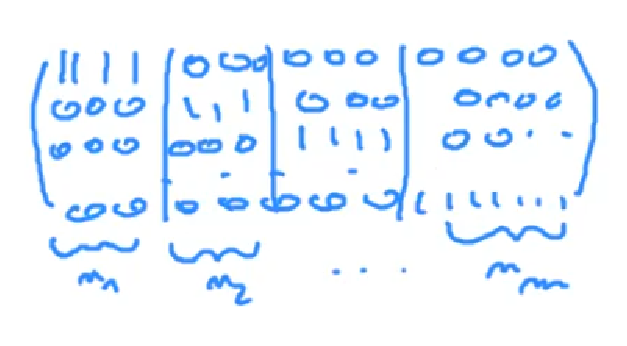
\includegraphics[scale=0.6]{sp_2.eps}

	Potom $PP^T$ je diagonální matice $D$ protože jedničky jsou na různých pozicích. Skalární součin dvou různých řádku je 0.
	Na diagonále je norma i-ho řádku $= n_i$.

	Použijeme matici $P$ abychom dostali řádkové součty matici $A$:\\
	V matici $PA$ dostaneme sloupcový součet po blocích. Pak v matici $PAP^T$ dostaneme součty všech prvku v blocích.

	Pro rovnost s matici $B$ ještě potřebujeme vydělit $n_i$. Na což použijeme $D^{-1}$ která má na diagonále $\frac{1}{n_i}$.
	\[ B = D^{-1}PAP^T \]

	Nechť $S = D^{-1/2}P. S$ je reálná matice, pro niž platí
	\[ SS^T = D^{-1/2}PP^T(D^{-1/2})^T = D^{-1/2}DD^{-1/2} = E \]

	Dle Vety o propletani A \cref{sp_cross_a}, vlastní čísla $SAS^T$ propletaji vlastní čísla A.
	\[ SAS^T = D^{-1/2}PAP^T(D^{-1/2})^T = D^{-1/2}DBD^{-1/2} = D^{1/2}BD^{-1/2} \]
	Pak $SAS^T$ a $B$ jsou podobné $\Rightarrow$ mají stejný spektrum.
	\[ Sp(SAS^T) = Sp(B) \]
\end{proof}

\begin{theorem}[Nezav množ v d-regulárním]
	Nechť $G$ je d-regulární graf o $n$ vrcholech s vlastní čísly $\lambda_1 \geq \lambda_2 \geq ... \geq \lambda_n \}$. Pak
	\[ \alpha(G) \leq n \frac{-\lambda_n}{d - \lambda_n} \]
\end{theorem}
\begin{proof}
	Nechť A je matice sousednosti grafu $G$.

	\[ Sp(A) = \{\lambda_1 = d \geq \lambda_2 \geq ... \geq \lambda_n \} \]
	\[ Sp(J) = \{n, 0^{n-1} \} \]

	Matice A, $J$ komutuji $\Rightarrow$ mají společnou ortonormální báze.
	\[ \exists X: X^{\ast}X = E, X^{\ast}AX = \Lambda_A \]
	Kde $\Lambda_A$ je diagonální matice s vlastní čísly na diagonále, rozmíštěné dle uspořádaní.
	Podobně pro $J$:
	\[ X^{\ast}AX = \Lambda_J, (\Lambda_J)_{1,1} = n \]

	Z věty o ortonormální bázi vlastní vektor příslušný největšímu vlastnímu číslu je nezáporný. Ostatní mají záporné složky.
	Pak vektor $\bar{1}$ je příslušný největšímu vlastnímu číslu A - $d$.
	Taky odpovídá vlastnímu číslu $n$ matice $J$.

 	Uvažme matici:
	\[ C = A - \frac{1}{n}(d - \lambda_n)J \]
	Její vlastní čísla jsou lineární kombinace vlastních čísel $A, J$.
	\[ X^{\ast}CX = X^{\ast}(A - \frac{1}{n}(d - \lambda_n)J)X = X^{\ast}AX - \frac{1}{n}(d - \lambda_n)X^{\ast}JX = \Lambda_A - \Lambda_K = \Lambda_C \]
	Kde $(\Lambda_K)_{1,1} = d - \lambda_n$, jinak 0. Z toho $\Lambda_C$ má na diagonále $\{ \lambda_n, \lambda_2,..., \lambda_n \}$.
	Odtud $\lambda_n$ je největší vlastní číslo matice $C$.

	Nechť $W \subseteq V(G)$ je nezávislá množina $G$, $|W| = \alpha(G)$. Pak matice $A$, po seskupeni řádku odpovídajících $W$, má nulovou hlavni podmatice odpovídající $W$.
	Z toho matice $C$ má na těchto pozicích $-\frac{1}{n}(d - \lambda_n)$. Taky je to hlavni podmatice.

	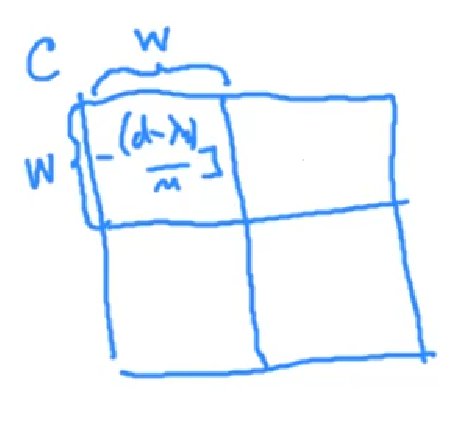
\includegraphics[scale=0.5]{sp_1.eps}

	Vlastní čísla matice $-\frac{1}{n}(d - \lambda_n)J$ propletaji vlastní čísla matice $C$.
	\[ Sp\left(-\frac{1}{n}(d - \lambda_n)J\right) = \{0^{\alpha - 1}, \alpha * -\frac{1}{n}(d - \lambda_n) \} \]
	Z vety o propletaní:
	\[ \alpha(G) * -\frac{1}{n}(d - \lambda_n) \geq \lambda_n \Rightarrow \alpha(G) \leq n \frac{-\lambda_n}{d - \lambda_n} \]
\end{proof}

\begin{consequence}\label{coloring_1}
	Nechť $G$ je d-regulární graf o $n$ vrcholech s vlastní čísly $\lambda_1 \geq \lambda_2 \geq ... \geq \lambda_n \}$. Pak
	\[ \chi(G) \geq 1 + \frac{\lambda_1}{|\lambda_n|} \]

	Plyne z toho, že $ \chi(G) \geq \frac{n}{\alpha(G)}$. Barveni grafu je rozložení na $\chi(G)$ nezávislých množin. Kazda z nich má velikost $\chi(G)/\alpha(G)$. Kombinaci dvou nerovnosti dostaneme tvrzení.
\end{consequence}

\begin{theorem}[Poloměr spektra grafu]\label{sp_polomer}
	Nechť $G$ je graf o $n$ vrcholech s vlastní čísly $\lambda_1 \geq \lambda_2 \geq ... \geq \lambda_n \}$. Pak
	\[ \Delta(G) \geq \lambda_1 \geq deg_{avg}(G) \]

	Kde $\Delta(G)$ je max $deg$ grafu.
\end{theorem}
\begin{proof}
	1) Nerovnost $\Delta(G) \geq \lambda_1$. Doplníme $G$ na $\Delta$-regulární graf $H$ tak, aby $G$ byl jeho indukovaný podgraf. Pak vlastní čísla $G$ propletaji vlastní čísla $H$. $\lambda_{max}(H) = \Delta \Rightarrow \Delta(G) \geq \lambda_1$.

	2) Nerovnost $\lambda_1 \geq deg_{avg}(G)$.
	Vezmeme matice sousednosti $A$, představíme ji jako matici s 1 blokem. Pak matice průměrných řádkových součtu je $B = deg_{avg}(G)$ jednoprvková.

	Dle Vety o propletaní B \cref{sp_cross_b}, $Sp(B) = \{ deg_{avg}(G)\}$ propleta spektrum A $\Rightarrow \lambda_1 \geq deg_{avg}(G)$.
\end{proof}

\begin{theorem}[Barevnost libovolného grafu]
	Nechť $G$ je graf o $n$ vrcholech s vlastní čísly $\lambda_1 \geq \lambda_2 \geq ... \geq \lambda_n \}$. Pak
	\[ \chi(G) \leq 1 + \lambda_1 \]
\end{theorem}
\begin{proof}
	Nechť $H$ je $\chi$-kriticky indukovaný podgraf grafu $G$. Minimální stupeň vrcholu v $\chi$-kritickém grafu je aspoň $\chi - 1$.
	Označme jeho největší vlastní číslo jako $h_1$. Z vety o propletaní plyne $\lambda_1 \geq h_1$.
	Z vety poloměru spektra \cref{sp_polomer} dostáváme
	\[ h_1 \geq deg_{avg}(H) \geq \delta(H) \geq \chi - 1 \Rightarrow \lambda_1 \geq \chi - 1 \]
\end{proof}

\begin{theorem}[Nezav množ v libovolnem grafu]
	Nechť $G$ je graf o $n$ vrcholech s vlastní čísly $\lambda_1 \geq \lambda_2 \geq ... \geq \lambda_n \}$. Pak
	\[ \alpha(G) \leq n \frac{-\lambda_1\lambda_n}{\sigma^2(G) - \lambda_1\lambda_n} \]
\end{theorem}
\begin{proof}
	Nechť $W \subseteq V(G)$ je nezávislá množina $G$, $|W| = \alpha(G)$. Rozdělíme matice $A$ dle $W$ a $V\setminus W$.

	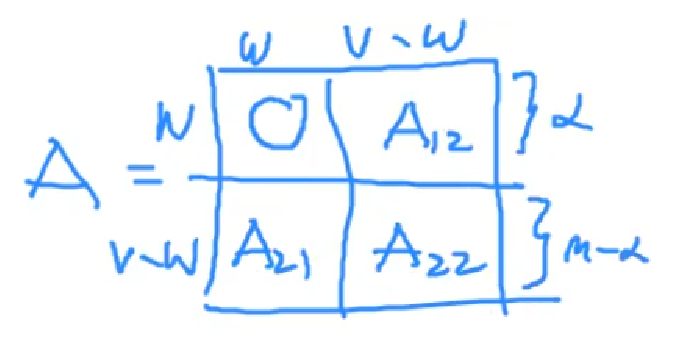
\includegraphics[scale=0.5]{sp_3.eps}

	Použijeme Vetu o propletaní B \cref{sp_cross_b}.
	\[ B =
	\begin{pmatrix}
		0 & b_{12}\\
		b_{21} & b_{22}\\
	\end{pmatrix}
	\]

	Pak $Sp(B) = \{ h_1 \geq h_2 \}$ propleta $Sp(A) = Sp(G)$.

	Dal víme, ze počet hran mezi $W$ a $v\setminus W$ se rovna
	\[ \alpha b_{12} = (n - \alpha) b_{21} \Rightarrow b_{21} = \frac{\alpha}{n - \alpha} b_{12}\]

	Z LA součin vlastních čísel je determinant:
	\[ h_1h_2 = det(B) = -b_{12} \cdot b_{21} = b_{12}^2 \cdot \frac{\alpha}{n - \alpha}\]

	Z propletaní:
	\[ \lambda_1 \geq h_1 \geq h_2 \geq \lambda_n \Rightarrow -h_2 \leq -\lambda_n \Rightarrow -h_1h_2 \leq -\lambda_1 \lambda_n \]

	Protože všichni sousede vrcholu z $W$ jsou z $V(G) \setminus W \Rightarrow b_{12} \geq \delta(G)$.
	\begin{gather*}
	-\delta^2(G) \frac{\alpha}{n - \alpha} \leq -\lambda_1 \lambda_n\\
	-\delta^2(G) \alpha \leq (n - \alpha) * (-\lambda_1 \lambda_n)\\
	\alpha(\delta^2(G) - \lambda_1 \lambda_n) \leq n(-\lambda_1 \lambda_n)\\
	\alpha(G) \leq n \frac{-\lambda_1\lambda_n}{\sigma^2(G) - \lambda_1\lambda_n}
	\end{gather*}
\end{proof}

\begin{theorem}[Barevnost souvislého grafu]
	Nechť $G$ je souvislý graf o $n$ vrcholech s vlastnímu čísly $\lambda_1 \geq \lambda_2 \geq ... \geq \lambda_n \}$. Pak
	\[ \chi(G) \geq 1 + \frac{\lambda_1}{|\lambda_n|} \]
	Veta je analogická důsledku vety 1 \cref{coloring_1}, zesiluje ji pro souvisle grafy.
\end{theorem}
\begin{proof}
	Obarvíme graf pomoci $\chi$ barev. Nechť $x$ je reálný vlastní vektor příslušný vlastnímu číslu $\lambda_1$ (Existuje dle Frobeniove vety).
	Ze souvislosti $x_i > 0 \forall i$.

	Sestavíme matici $P \in \Real^{\chi \times n}$.
	\[ P_{ij} = \twopartdef{ x_j} {j \in W}{0}{j \notin W} \]
	Pak $PP^T = D$ je diagonální matice, na diagonále $\sum_{u \in W_j}x_u^2 > 0$.
	Nechť $S = D^{-1/2}P$.
	Protože
	\[SS^T = D^{-1/2}PP^T(D^{-1/2})^T = D^{-1/2}DD^{-1/2} = I\]
	Dle Vety o propletaní A \cref{sp_cross_a}, vlastní čísla $SAS^T$ propletaji vlastní čísla A.
	Nechť vlastní čísla $SAS^T$ jsou $\{h_1, h_2,..., h_{\chi} \}$. Má na diagonále samé nuly, z toho %todo rozbit dle bloku
	\[ \sum_0^{\chi} h_i = 0 \]

	Dal
	\[ SAS^{T}D^{1/2} \cdot \bar{1} = SAP^TD^{-1/2}D^{1/2} \cdot \bar{1} = SAP^T \bar{1} \]

	\[ P^T \cdot \bar{1} = x \Rightarrow SAP^T \bar{1} = SAx = \lambda_1 Sx = \lambda_1 D^{-1/2}PP^T \bar{1} = \lambda_1 D^{-1/2}D \bar{1} = \lambda_1 D^{1/2} \bar{1} \]
	Dostáváme
	\[ SAS^TD^{1/2} \cdot \bar{1} = \lambda_1 D^{1/2} \bar{1} \Rightarrow \lambda_1 \in Sp(SAS^T) \]
	Ale taky odpovídá nenulovému reálnému vlastnímu vektoru, takže $\lambda_1 = h_1$.
	Použijeme propletani
	\[ h_1 = \lambda_1 \geq h_2 \geq ... \geq h_{\chi} \geq \lambda_n \land \sum h_i = 0 \Rightarrow -\lambda_1 = h_1 = -\sum_2^{\chi} h_i \]
	Použijeme horní odhad pro součet přes \# sčítanců krát min hodnota ($\lambda_n$).
	\[ -\lambda_1 = h_1 = -\sum_2^{\chi} h_i \geq (\chi - 1)(-\lambda_n) \]

	Po upravě
	\[ \chi(G) \geq 1 + \frac{\lambda_1}{|\lambda_n|} \]
\end{proof}
